\chapter{Study Design}\label{chapter:studydesign}
The main goals of this thesis were to develop an exergame which can be used for warm up routine before more strenuous physical activity and to evaluate its effectiveness in terms of guiding the user through the process of warming up. In this chapter we outline the research framework, detail the research methods and present the obtained results.
\section{Description of the Experiment}
This section describes the evaluation of the second version of the Immotion exergame. For this purpose, an approach was adopted that uses a mixture of different tools and user study methods. During this period, data has been logged, surveys have been conducted, and interviews undertaken. Similarly to the evaluation of the prototype exergame (Chapter 2), the obtained results are analyzed in order to determine to which level our proposed solution was effective in the given context and whether it offered a solution to the problem. %Based on the results from the exergame prototype evaluation (Chapter: Implementation) and a variety of research presented (Chapter Related Work), guidelines were followed which influenced the design and development of the second version of the Immotion exergame. 

\subsection{Introduction and Goals} \label{chapter:goals}
%II. AIMS
%The objectives of this research were to answer the
%following questions:
%A. How do sixth form students percieve gamification in CPR
%teaching?
%B. Does teaching CPR to sixth form students using direct
%feedback manikins change student’s attitudes towards:
%1) Confidence in performing CPR and use of an
%Automated External Defibrillator (AED)?
%2) Willingness to perform CPR and use an AED?
%3) Perceived competence in performing CPR and using an
%AED?
%C. Can we promote healthy living through CPR training?
%The overall aim of the project is to introduce students to
%CPR training using mobile uploads of scores, direct feedback
%via the CPR manikin and gamification through a competitive
%online leaderboard and increasing difficulty levels. The
%information gathered will help establish how best to use these
%techniques when teaching CPR in schools and will be used to
%set up a yearlong project in the schools to teach CPR.%

The first study evaluated the prototype exergame. Based on the results obtained, comments, and suggestions, the prototype exergame has been modified to better suit the needs of its future users. The primary goal of the second study was to investigate whether our exergame solution can be used as an interactive guide for individuals who do not know how to perform warm up routines. In addition, we examined if the exergame can be used as a solution that motivates individuals to warm up before physically more demanding exercises, and provides an enjoyable game experience. Taking this into account, the research questions we address in this study are as follows: 
\begin{enumerate}
\item \textbf{RQ1: Evaluation of effectiveness} - How effective our proposed solution is in guiding the user through the warm up routine compared to the guidance offered by classic (traditional) methods?
%\item Comparing the experience between participants that use the exergame and participants that do not use the exergame. 
%\item Can our proposed solution motivate individuals to undertake warm up procedure?
\item \textbf{RQ2: Evaluation of perceived usefulness and ease of use} - How useful and easy to use our proposed solution is?
\item \textbf{RQ3: Evaluation of the usability} - How usable our proposed solution is? 
\item \textbf{RQ4: Evaluation of the game experience} - How enjoyable and entertaining our proposed solution is? 
\end{enumerate}
%The actual warm up was the original procedure:  
%\begin{itemize}
%\item The warm up routine was derived from sports literature.
%\item The exergame has been designed with this in mind.
%\item A video has been recorded with the original procedure.
%\end{itemize}http://edutechwiki.unige.ch/en/Usability_and_user_experience_surveys
%http://www.nigelbevan.com/papers/What_is_the_difference_between_usability_and_user_experience_evaluation_methods.pdf
In order to evaluate the effectiveness, perceived user experience, usefulness and usability of our gamified solution in the given context, the user base is divided into two groups: \textit{experimental group} and \textit{control group}. The first, experimental group, is the one that interacts with the exergame directly. Contrarily, the control group is presented with the video of a coach (professional) who guides the participant through the warm up routine. This division allows us to infer the influence of our gamified solution, as well as, to assess the main differences in completing the required activities between the two user groups. 
%\subsubsection{Assumptions}
%\begin{itemize}
%\item The participants will be able to perform the requested movements.
%\item The participants will answer all the questionnaires truthfully.
%\item The software and hardware that is used used will function properly.
%\end{itemize}
\subsubsection{Hypotheses}
%Remember to state these in terms of the independent and dependent variables. If it is not immediately clear why you would have a certain hypothesis (it often follows logically from the introduction of the experiment), then include a brief explanation separate from but following the hypothesis. You do not need to state the null hypothesis.%
Based on the research questions outlined in the previous section, the following hypotheses are established to be tested: 
\begin{enumerate}
\item The exergame itself is sufficient for guiding the player through a proper warm up procedure with correct movements. 
\item After the warm up routine is completed using the exergame, the player reached a significantly higher increase in ROM.
%\item Participants that are interactively guided through the warm up procedure using the exergame have perceived exertion during physical activityexertion during a testperceived user experience in terms of PRC scale, compared to the participants who warm up without the exergame.
\item Participants had a more positive perceived warm up experience when using the exergame compared to the participants not using the exergame.  
%\item Participants can easily follow the exergame and perform all the required movements. MODIFY %felt more motivated to undertake warm up exercises when using the exergame compared to the participants not using the exergame.
%\item The exergame will encourage more 
%behavior change compared to the standard warm up %procedure. - for longer study
\end{enumerate}
\pagebreak
%Introduce your experiment, and give the reader the specific goals you expect it to address. It is common at this stage to give the reader a hint of your hypotheses (if they are not already hinted at in the Introduction).%
\subsubsection{Apparatus}
The experiment was conducted in the laboratory room in DFKI on (add date). The laboratory is presented in Figure \ref{fig:lab1}.\\ 
\begin{figure}[h]
    \centering
    \includegraphics[width=0.9\textwidth]{Room1}
    \caption{Laboratory.}
    \label{fig:lab1}
\end{figure}\\
The following equipment has been used during the experiment:
\begin{itemize}
\item Kinect for Xbox One (2.0 2013) motion sensing input devices by Microsoft used for movement detection and controlling the exergame avatar. 
\item PC running the game engine.
\item Projector used to display the game (video) on the wall in front of the participant.
\item Microsoft Band used for gathering heart rate data.
\item Goniometer used for measuring participants' ROM.
\end{itemize}\pagebreak
The Kinect motion sensor has been placed in front of the display panel facing the participant playing the exergame. The participant was instructed to keep at least 2 meter distance from the sensor during the gameplay. This distance was the most optimal in order to ... The sensor is presented in Figure \ref{fig:kinect}.\\
\begin{figure}[h]
    \centering
    \includegraphics[width=0.9\textwidth]{Kinect}
    \caption{Kinect motion sensor.}
    \label{fig:kinect}
\end{figure}\\
We used XXX beamer in order to project the exergame to the display. The beamer, showed in Figure \ref{fig:projector} was placed above the user so it did not interfere with the game flow. The desktop set up that consisted of XXX is presented in Figure \ref{fig:desktop}.\\
\begin{figure}[h]
    \centering
    \includegraphics[width=0.9\textwidth]{Desktop}
    \caption{Desktop set up.}
    \label{fig:desktop}
\end{figure}
\begin{figure}[h]
    \centering
    \includegraphics[width=0.9\textwidth]{Projector}
    \caption{Projector.}
    \label{fig:projector}
\end{figure}
\subsection{Methods} 
In this section we outline the methodology adopted for the Immotion exergame evaluation. For this purpose we utilize the traditional (moderated) usability test since it gives direct input on how real users use the system. %First, we measure users' performance. That is, we measure the time users' will spend performing the warm up exercises with the exergame and with the video. The amount of time users' feel warmed up sufficiently. 
%We decide to follow a mixed-methods approach, and by doing so, utilize both qualitative and quantitative data sources in combination. Second, we measure users' satisfaction level. What the user thinks about his interaction with the product (visually appealing) 
%
%This is a detailed description of the experiment that should allow other researchers (familiar with HCI and experimental design in general, but not familiar with your experiment) to replicate your experiment.%
\subsubsection{Participants}
Demographic details of the participants to be added when the study is completed.\\
Total of n = X individuals participated in the study that has been conducted DATE in DFKI. All participants were students from Saarland University. For recruiting participants, posters were distributed in print, and sent through social media and email (Appendix X). Each participant was given X euros for taking part in the study. All of the participants were amateur athletes who engage in some physical activity on average X times per week. For the study we particularly targeted individuals who exercise in gym or fitness centers and often avoid preforming warm up exercises before more strenuous physical activity. All participants were required to report to the laboratory in gym based clothing, preferably shorts and t-shirt, and all of them performed the required tests in the same location using the same equipment. Before the study, each participant signed a consent form (Appendix X). TODO: This should be updated later with real data.
%Describe your participants (e.g., any relevant demographics, if/how they were divided into categories), including total number, and recruiting approach. Indicate if any incentives were used. Comment on the representativeness of your participants relative to the target population, if their representativeness isn’t immediately obvious.%
\subsubsection{Conditions}
First 20 participant who applied for the experiment have been accepted. These participants were sent a pre-test questionnaires (\acrshort{bsa}, \acrshort{parq}, and Demographic questionnaire) that needed to be completed before coming to the experiment. Based on the answers given, the participants were assigned to the control or the experiment group. Each assigned participant took part in a single test session one hour in duration. During this session, all the participants  performed one warm up session, after which they completed a set of questionnaires. Two conditions were evaluated:
\begin{enumerate}
\item Warming up with the exergame guiding through the warm up procedure, projected on a wall in front of the participant.
\item Warmin up with a video of a professional (coach) guiding through the exact same warm up procedure as induced by the exergame, projected on a wall in front of the participant.
\end{enumerate}
Depending on the group, each participant performed exercise that represent one of the conditions.
\subsubsection{Control and Experiment Groups}
The participants are assigned to each group based on the previously completed self-reported questionnaires. These questionnaires were sent to each participant and needed to be completed before the experiment. Based on the answers provided, each participant was assigned to either control or experiment group. The surveys assessed participants' perceived physical fitness level, warm up preferences, and previous exergames experience.
\subsubsection{Measures and Metrics}
%All tasks were performed under a cognitive walkthrough approach, and all data was
%recorder. After performing the tasks, and taking the CUE-model [12] as a framework and
%following adaptations already mentioned in literature review (cf. ([13]; [14];[15]; [16]), three
%instruments were used in order to assess the users’ perspectives about the applications’
%instrumental and non-instrumental qualities, and the user’s emotional reactions to the whole
%experience.
%For assessing the applications’ instrumental qualities (e.g. controllability, effectiveness,
%learnability), the research team used the SUS - System %Usability Scale [17] and the
%Pragmatic dimension of AttrakDiff [18]. The SUS-scale [17] is %a 10-item questionnaire with a
%5-point Likert scale developed to assess several usability aspects such as ease of use and
%usefulness. As for AttrakDiff [18], it is an instrument created to measure the attractiveness of
%an application by presenting the user/evaluator three groups of opposite adjectives.
%AttrakDiff records both the perceived pragmatic quality, the hedonic quality and the
%attractiveness of an interactive product or application.
%For accessing non-instrumental qualities (e.g. aesthetics, identification) the research team
%used the AttrakDiff Hedonic dimension.
%Finally, for the evaluation of emotional reactions (e.g. valence, arousal, control of the
%application), the research team used the SAM - Self-assessment Manikin [19]. The
%SAM-Manikin is a non-verbal pictorial assessment method that directly assesses the
%pleasure, arousal, and dominance associated with the user’s affective reactions to a certain stimuli.
%Qualitative data was also collected through a semi-structured interview conducted at the end
%of the test session, aiming to get the participant’s opinion regarding the application (its main
%features), the interface and the adopted solutions
Two separate sets of questionnaires were administered, one
prior to the experiment session and one post the session in order to gather self-reported user perception data.
The pre-test questionnaires focused on participants' demographic information, overall physical and psychological abilities, hours spent on exercise, frequency and activity
of warm up procedures, extent of video gameplay, and reason for playing. The pre-test questionnaires were as follows:
\begin{itemize}
\item \textit{Physical activity screening}. Pre-study physical activity levels have been assessed with a standardized questionnaire  \gls{bsa} \cite{fuchs2015messung}. Participants were instructed to indicate for how many minutes per week they performed everyday physical activities (e.g., taking the bike to work; taking a walk) in average during the last four (TODO: discuss the time frame) weeks. 
\item \textit{Health status}. The current health status of the participants has been assessed via the \gls{parq}, which consists of seven dichotomous items \cite{thomas1992revision}. The individual response patterns were used in order to assess if participants were physically able to perform the warm up session.
\item Demographic survey with included questions regarding warm up preferences, and previous exergame experience [Appendix].
\end{itemize}
The second set of questionnaires have been administered after the completion of the warm up procedure. In these questionnaires participants' level of exertion, emotional state, and game experience have been assessed. The questionnaires were as follows:
\begin{itemize}
\item \textit{Perceived exertion}. For assessing the perceived exertion of the warm up session, the \gls{rpe} has been utilized \cite{borg1998borg}. The perceived exertion reflects how difficult and strenuous the performed warm up exercise feels to the participants, combining all sensations and feelings of physical stress, effort, and fatigue.
\item \textit{Emotional state}. The pleasure, arousal, and dominance associated with a person's affective reaction to a wide variety of stimuli has been assessed with \gls{sam} \cite{bradley1994measuring}. 
\item \textit{Enjoyment of the physical activity}. To test the enjoyment of the physical activity performed, in this case the warm up procedure, the \gls{paces} has been used \cite{kendzierski1991physical}. 
\item \textit{System usability}. For assessing the exergame's instrumental qualities (e.g. controllability, effectiveness, learnability), the \gls{sus} has been used.
\item \textit{Enjoyment of digital games} In order to measure the enjoyment of digital games the \gls{geq} has been utilized. It is a general questionnaire with the goal of being able to be applied to any game regardless of genre or mechanics in order to measure their users' experience.
\end{itemize}
(TO BE DISCUSSED: Sport oriented questionnaire (SOQ), Task and Ego Orientation in Sport Questionnaire (TEOSQ), AttrakDiff, User Experience, Exergame Experience questionnaires are also used in some studies.)\\
During the experiment, the following metrics were collected from each participants:
\begin{itemize}
\item \textit{Range of motion}. The participants' ROM has been measured before and after the warm up routine using goniometer. (TODO)
\item \textit{Heart rate}. The participant's heart rate data has been captured and the measured during the warm up procedure using Microsoft Band.
\item \textit{Distance}. The overall distance the participants' moved during the warm up routine was measured using Microsoft Kinect. 
\end{itemize}
%The warm up routine performed by the participant has been recorded using Canon XXX camera for further analysis of performed movements during the warm up procedure.
%If your experiment is comparing multiple different interfaces or interactive systems or techniques, describe each of them. Screen snapshots of interfaces/systems are particularly useful.%
\subsubsection{Tasks}
In order to interact with the gamified system, the participants in the experiment group were required to perform a set of general movements. By performing these movements, the participant controlled the game avatar and, by doing so, avoided obstacles and collected coins. Based on the data and feedback gathered from the first study, we limited the movements the participants need to perform in the exergame. That is, only movements that are detectable with high accuracy using only one Kinect device and simplistic enough to be accomplished easily without no prior exercise knowledge or experience were required. These movements were: 
\begin{itemize}
\item right hand movement up,
\item left hand movement up,
\item jump right,
\item jump left,
\item jump up, 
\item star jump, and
\item squat.
\end{itemize}
Participants who were in the control group and did not interact with the gamified system were required to perform the same set of general movements. However, participants in this group had to follow a video that was projected on the wall in front of them. The video was a recording of a professional (coach) who guided the participants through the warm up routine. By following the video, and thus the coach, the participants were required to execute the same movements as the participant in the experiment group who interacted with the exergame.
%Briefly describe what participants were asked to do with the interactive system(s).%
%\subsubsection{Design}
%TO DISCUSS this section. Write the formal experimental design (e.g., a 2 x 3 mixed factorial design, more specifically a 2 levels of expertise (between subjects) x 3 interfaces (within subjects) design). 
\subsubsection{Procedure}
%Describe the sequence of activities each participant followed. This should document the experiment from a participant’s perspective, from the moment s/he arrives (e.g., a preliminary questionnaire to obtain X information, followed by five tasks with system A, then a 10 min break, followed by the same five tasks with system B, and finally a semi-structured interview to solicit opinion on Y).%
%The activities each participant of the experiment session followed is presented in this section.\\ 
The study protocol was reviewed and approved by an institutional ethics committee. For data collection, we used a  paper and pencil as well as \textit{Google forms} questionnaires.
Before the experiment, the lab environment is set up. The Kinect sensor is placed in a correct position and turned on. The PC running the software is started and the projector is enabled. In each session only one participant was present and guided by the researcher. The activities each participant followed are:
\begin{itemize}
\item The participant completes the preliminary survey.
\item The researcher explains the sensors and tools that are required for the experiment, after which the participant puts them on. 
\item After the researcher confirms that the sensors are placed in a correct position, we start recording heart rate data.
\item The researcher measures the participant's ROM before starting the warm up procedure for the following joints: (TODO decide which joint will be measured).
\item After the measurements are completed, the participant rests.
\item The researcher gives a general explanation on the benefits of a proper warm up routine before physically more demanding exercise.
\item The participant moves to the spot marked by the researcher.
\item The researcher starts recording the session. 
\item The warm up procedure begins:
\begin{itemize}
\item If this participant is part of the experimental group, the game starts with the start scene where the participant enters his or her name. After 5 seconds, the game proceeds with scenes in which the participant performs specific movements in order to avoid obstacles and collect coins. The duration of the game is not fixed and it is played up to the point when the participant feels warmed up enough. 
\item  In case the participant is part of the control group, the video that displays a coach who instructs the participants which movements need to be performed. As with with the sessions in the experiment group, the duration of the warm up is not fixed and the video is played up to the point when the participant feels warmed up enough.
\end{itemize}
\item After finishing with the warm up routine, the participant takes a rest. During this period the researcher assesses the ROM of the participant. 
\item After taking the ROM measures, the sensors are removed.
\item The participant completes the post-test surveys . %https://www.verywell.com/rating-of-perceived-exertion-scale-3119445
\end{itemize}
\subsubsection{Independent and Dependent Variables}
Include exactly how you intend to measure each dependent variable. 
%https://books.google.de/books?hl=de&lr=&id=bPhLeMBLEkAC&oi=fnd&pg=PP1&dq=measuring+the+user+experience&ots=R9KdcqS-vF&sig=2-V-FaMOeX24Rn0pG30lWVdvjSo#v=onepage&q=measuring%20the%20user%20experience&f=false
Independent variables are the things you manipulate or control for, such as design's you are testing or the ages of the respondents. 
Dependent variables are the things you measure, such as success rate, number of errors, user satisfaction, completion time, and many more. Have s clear idea what do you manipulate - independent variables, and what do you want to measure - dependent variables. The most interesting is the intersection - is one design results in a higher task success rate than other. 

Independent and dependent variables can be measured by 4 types of data: nominal, ordinal, interval, and ratio. 
Nominal (categorical) data: groups or categories. Mac vs Windows users, male vs female. These are independent variables, that allows you to segment data by these different groups. Nominal data also includes dependent variables like task success, number of users who clicked link A instead B... 
Ordinal: ordered data - imdb. In user studies this comes from self-reported data. User states if someone is good better worse... These are relative rankings. You report it by frequencies: for example 40 percent said it is good. 

\subsection{Problems/Limitations - Threats to Validity}
Describe any problems/limitations encountered that will help other researchers avoid or account for them if they decide to replicate your experiment.
\section{Results}

This section is an objective report on what the numbers show. You should not try to interpret the meaning of the numbers in this section. Some of the things you may do here are: 
report means and standard deviations in neat tables 
indicate the statistics used and levels of significance 
include graphs, plots, histograms, etc that tell a story about the actual figures obtained 
Only critical raw data and summary statistics should be included in the actual report. However, you must keep all your raw data in a separate archival report, should anyone (a reviewer in the case of real scientific reporting) need more detail than is provided in the paper. 
\section{Discussion}
Interpret the results. Although you should still try to be as objective as possible, the discussion section should illuminate your critical thinking about the results. Explain what the statistics mean, account for anomalies, and so on.
\subsection{Interpretation of Results}
Discuss what you believe the results really mean. For example, if you find a significant difference for some effect, what does that mean to the hypothesis? Is the different seen an important one?
\subsection{Relation to other works}
How do the results you’ve obtained relate to other research findings?
\subsection{Impact for practitioners}
As computer scientists, we are particularly concerned with the implications of our findings on practitioners. Should existing interface constructs be designed differently or used in a new context? Do you have suggestions for new designs? How can the findings be generalized?
\subsection{Critical reflection}
Critical reflection is one of the key foundations of science. You should criticize your work (constructively, if possible), indicate possible flaws, mitigating circumstances, the limits to generalization, conditions under which you would expect your findings to be reversed, and so on.
\subsection{Research agenda}
The best experiments suggest new avenues of exploration. In this section, you should reflect and refine your hypotheses, describe new hypotheses, and suggest future research, ie research that you would do if you continued along this path.
\section{Conclusions}
Summarize the report, and speculate on what is to come.
Acknowledgements. This section should give thanks to the major people (supervisors, associates) and organizations (sponsoring agencies, funders) that helped you. For example, I would like to thank Ben Shneiderman, whose report framework was used to build this one.

\begin{appendices}
  \chapter{Self-Assessment Manikin Scale}
  \centering
  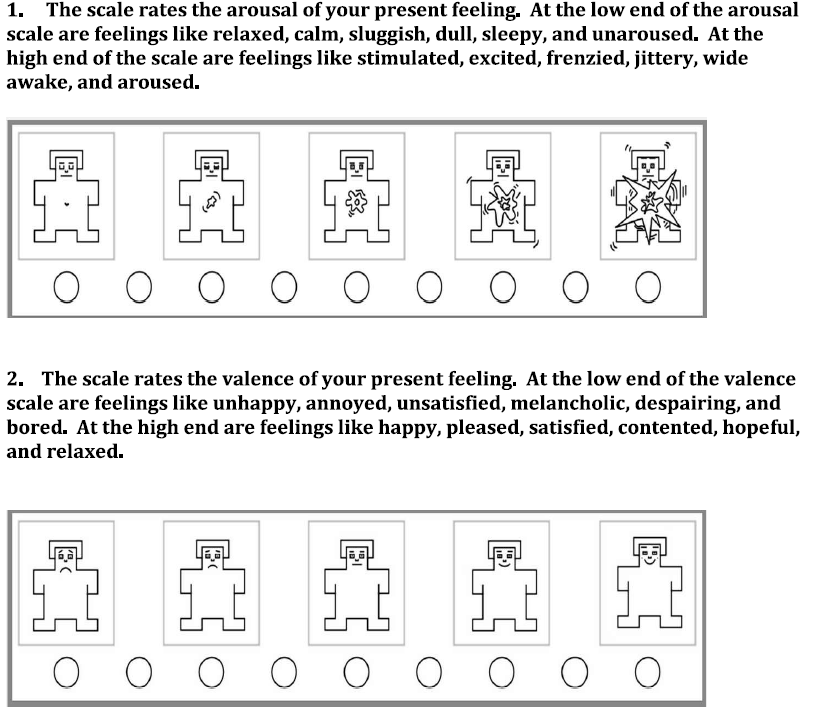
\includegraphics[width=\textwidth]{manikin}
  \label{appendix:sam}
\end{appendices}